%
% Modo de operación OFB, capítulo de antecedentes.
% Proyecto Lovelace.
%

\newpage
\subsection{\textit{Output Feedback} (OFB)}

Este es muy similar al anterior (CFB), salvo porque la retroalimentación va
directamente de la salida del cifrador a bloques. De esta forma, nada que
tenga que ver con el texto en claro, llega al cifrado a bloques; este
solamente se la pasa cifrando una y otra vez el vector de inicialización.

\vspace{0.5cm}

\begin{figure}[H]
  \centering
  \begin{subfigure}{0.45\textwidth}
      \begin{center}
          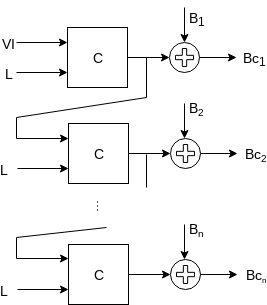
\includegraphics[width=0.7\linewidth]
            {contenidos/antecedentes/modos/diagramas/modo_ofb.png}
          \caption{Cifrado.}
      \end{center}
  \end{subfigure}
  \begin{subfigure}{0.45\textwidth}
      \begin{center}
          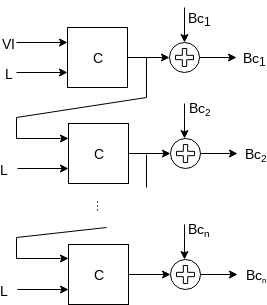
\includegraphics[width=0.7\linewidth]
            {contenidos/antecedentes/modos/diagramas/modo_ofb_inverso.png}
          \caption{Descifrado.}
      \end{center}
  \end{subfigure}
  \caption{Modo de operación OFB.}
\end{figure}

\begin{pseudocodigo}[caption={Modo de operación OFB (cifrado y descifrado).}]
  entrada: llave $ L $; vector de inicialización $ VI $;
           bloques de mensaje (cifrado o descifrado) $ B_1, B_2 \dots B_n $.
   salida: bloques de mensaje (cifrado o descifrado) $ Bc_1, Bc_2 \dots Bc_n $.
  inicio
    auxiliar $\gets$ $ VI $
    para_todo $B$
      auxiliar $\gets$ C($L$, auxiliar)
      $Bc_i$ $\gets$  auxiliar $\oplus$ $B_i$
    fin
    regresar $Bc$
  fin
\end{pseudocodigo}
